\documentclass[10pt,letterpaper]{article}
\usepackage[margin=0.67in,top=0.62in,bottom=0.62in,headheight=20pt,headsep=12pt,footskip=22pt]{geometry}
\usepackage[T1]{fontenc}
\usepackage{newtxtext,newtxmath}
\usepackage[scaled=0.92]{helvet}
\usepackage{microtype,multicol,booktabs,graphicx,xcolor,tikz,caption,fancyhdr,titlesec,enumitem}
\usetikzlibrary{arrows.meta,positioning,calc}
\definecolor{ink}{HTML}{202B36}
\definecolor{blue}{HTML}{265878}
\definecolor{muted}{HTML}{566675}
\definecolor{rulegray}{HTML}{D5DDE3}
\definecolor{lightblue}{HTML}{F0F5F8}
\usepackage[colorlinks=true,urlcolor=blue,citecolor=blue,linkcolor=blue,pdfauthor={Zhijing Wu},pdftitle={When Performance-Equivalent Programs Differ Under Edits}]{hyperref}
\renewcommand{\normalsize}{\fontsize{10.5}{12.7}\selectfont}
\normalsize
\color{ink}
\setlength{\columnsep}{0.27in}
\setlength{\parindent}{0pt}
\setlength{\parskip}{4.2pt}
\setlength{\multicolsep}{6pt}
\raggedcolumns
\titleformat{\section}{\sffamily\bfseries\fontsize{11}{13}\selectfont\color{blue}}{\thesection}{0.5em}{}
\titlespacing*{\section}{0pt}{7pt}{3pt}
\captionsetup{font={small},labelfont={bf,color=blue},labelsep=period,skip=4pt,hypcap=false}
\pagestyle{fancy}\fancyhf{}
\fancyhead[L]{\sffamily\fontsize{8}{10}\selectfont\color{muted}INDEPENDENT RESEARCH NOTE\enspace /\enspace 20 OCTOBER 2026}
\fancyhead[R]{\sffamily\fontsize{8}{10}\selectfont\color{muted}ZHIJING WU}
\fancyfoot[L]{\sffamily\fontsize{8}{10}\selectfont\color{muted}Exploratory study motivated by MetaMuse}
\fancyfoot[R]{\sffamily\fontsize{8}{10}\selectfont\color{muted}\thepage\,/\,2}
\renewcommand{\headrulewidth}{0.3pt}
\renewcommand{\headrule}{\hbox to\headwidth{\color{rulegray}\leaders\hrule height \headrulewidth\hfill}}
\newcommand{\cost}{\mathcal{C}}
\newcommand{\refentry}[2]{\par\hangindent=1.55em\hangafter=1\noindent\makebox[1.55em][l]{[#1]}#2\par}
\begin{document}
\thispagestyle{fancy}
{\sffamily\bfseries\fontsize{19.5}{22}\selectfont\color{ink}
When Performance-Equivalent Programs Differ Under Edits:\\[2pt]
A Controlled Study of Search Representation and Retention\par}
\vspace{5pt}
{\sffamily\fontsize{11}{13}\selectfont\textbf{Zhijing Wu}\quad Sichuan University\par}
{\sffamily\fontsize{9}{11}\selectfont\color{muted}\href{mailto:zhijingwu.cs@gmail.com}{zhijingwu.cs@gmail.com}\enspace\textbar\enspace\href{https://zhijingwu.github.io/}{zhijingwu.github.io}\enspace\textbar\enspace\href{https://github.com/ZhijingWu}{github.com/ZhijingWu}\par}
\vspace{5pt}
\textbf{Finding.} Equal measured performance can hide different edit responses, but buying response information did not improve discovery in this controlled study. A completed 32-attempt comparison tied neutral retention at higher estimated generation cost. This independent undergraduate exploration establishes neither a new selection algorithm nor an official MetaMuse reproduction.

\begin{center}
% Original vector diagram. Illustrative symbols, no synthetic empirical values.
% Compile by input from the note; colors and TikZ libraries are defined there.
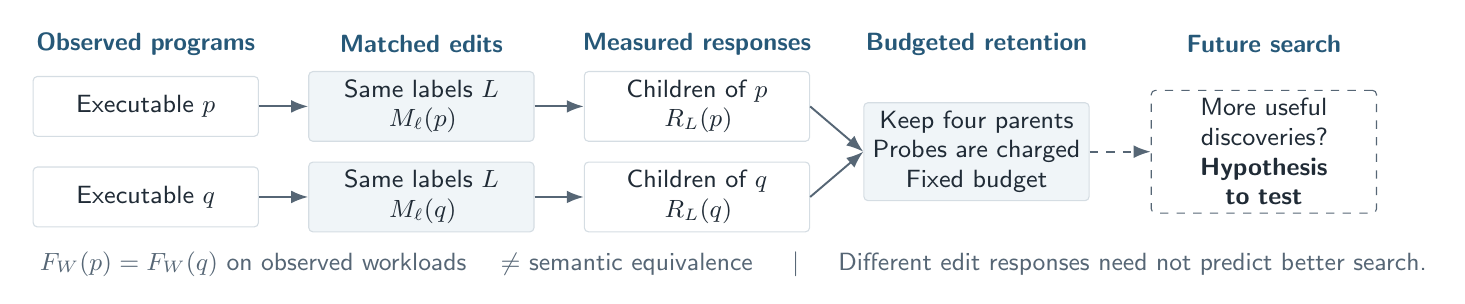
\begin{tikzpicture}[x=1cm,y=1cm,>=Latex,
  every node/.style={font=\sffamily\fontsize{9.2}{10.7}\selectfont,text=ink},
  box/.style={draw=rulegray,rounded corners=1.5pt,fill=white,align=center,minimum height=0.76cm,text width=2.65cm,inner sep=3pt},
  arr/.style={->,draw=muted,line width=0.7pt}]
\path[use as bounding box] (0,-0.1) rectangle (17.9,3.05);
\foreach \x/\label in {1.5/Observed programs,5.0/Matched edits,8.5/Measured responses,12.05/Budgeted retention,15.7/Future search}
  \node[font=\sffamily\bfseries\fontsize{9.2}{11}\selectfont,text=blue] at (\x,2.84) {\label};
\node[box] (p) at (1.5,2.05) {Executable $p$};
\node[box] (q) at (1.5,0.90) {Executable $q$};
\node[box,fill=lightblue] (ep) at (5.0,2.05) {Same labels $L$\\$M_{\ell}(p)$};
\node[box,fill=lightblue] (eq) at (5.0,0.90) {Same labels $L$\\$M_{\ell}(q)$};
\node[box] (rp) at (8.5,2.05) {Children of $p$\\$R_L(p)$};
\node[box] (rq) at (8.5,0.90) {Children of $q$\\$R_L(q)$};
\node[box,fill=lightblue,minimum height=1.16cm] (ret) at (12.05,1.475) {Keep four parents\\Probes are charged\\Fixed budget};
\node[box,draw=muted,dashed,text width=2.65cm,minimum height=1.16cm] (future) at (15.7,1.475) {More useful discoveries?\\\textbf{Hypothesis to test}};
\draw[arr] (p)--(ep);\draw[arr] (q)--(eq);
\draw[arr] (ep)--(rp);\draw[arr] (eq)--(rq);
\draw[arr] (rp.east)--(ret.west);\draw[arr] (rq.east)--(ret.west);
\draw[arr,dashed] (ret)--(future);
\node[anchor=west,font=\sffamily\fontsize{8.8}{10.5}\selectfont,text=muted] at (0.02,0.05)
  {$F_W(p)=F_W(q)$ on observed workloads \quad $\ne$ semantic equivalence \hspace{8pt} $\vert$ \hspace{8pt} Different edit responses need not predict better search.};
\end{tikzpicture}

\captionof{figure}{The question, not a validated mechanism. Solid arrows describe the probe-and-retain procedure; the dashed arrow marks the unverified hypothesis that retention improves future search. All program/response symbols are illustrative.}
\end{center}

\begin{multicols}{2}
\section{Motivation and testable distinction}
MetaMuse [1] steers creative algorithm generation with measured workload-performance diversity, external stimuli and waypoint reasoning. A follow-up question is whether two representations with equal current scores offer different opportunities for later edits. This is not a claimed MetaMuse bug: equal performance is not semantic equivalence, and MetaMuse need not identify the two.

Let $F_W(p)$ be a program's cost vector on observed workloads $W$, and $M_\ell$ a fixed labeled edit. The tested descriptor concatenates signed changes:
\[
R_L(p)=\mathop{\mathrm{concat}}_{\ell\in L}
\bigl[F_W(M_\ell(p))-F_W(p)\bigr].
\]
The claims are separated: equal measured performance; different edit responses; prediction of useful independent descendants; and better discovery \emph{after paying for probes}. Only the last justifies response-aware retention. Different stochastic samples alone do not establish different LLM mutation distributions.

\section{From exhaustive grammar to real edits}
\textbf{CPU study.} A finite grammar enumerated 625 scalar bin-priority programs. On 12 training traces, 5,628 of 5,655 same-performance pairs (99.52\%) had different uniform one-step mutation kernels over performance cells. These were grammar-generated programs, not LLM discoveries. An initial response selector tied random and structural controls; a collision-triggered revision lost to cheap neutral retention. The phenomenon did not validate a selection method.

\textbf{Interrupted LLM pilot.} GLM-4.7 produced 59 responses from 60 attempts, with 58 executable under the restricted interface. One training-selected child improved cost on the original 12 test traces from 7.2614 to 6.9882: one fewer bin on two traces, ten ties. A transport failure interrupted the planned full comparison. Its classification remains \textbf{INCONCLUSIVE}; unequal available pools cannot establish a response-selection advantage.

\section{Fresh, completed conditional comparison}
Eight human seeds form four equivalent pairs: Best Fit, First Fit, Worst Fit and target-residual fit. Code returns a stateless scalar priority for each feasible bin; a new bin opens only when none fits. Capacity is 100. A bounded AST interpreter enforces the contract. The metric is mean percentage excess over the volume lower bound:
\[
\cost_W(p)=\frac{1}{|W|}\sum_{w\in W}
100\,\frac{B(p,w)-L_w}{L_w},\quad
L_w=\left\lceil\frac{\sum_i x_{wi}}{100}\right\rceil.
\]
Lower is better; differences are percentage points (pp).

Revised selectors were frozen before fresh acquisition and testing. Sixteen old probes were reused \emph{with their original costs charged}; 64 new future requests supplied eight edits per parent, balanced across two labels. Old future children were excluded from search. All 64 requests returned, 58 were executable, and no transport retry occurred. Generation used GLM-4.7, temperature 0.9, thinking disabled and a 1,200-token output cap.

Each policy retains four parents and receives 32 attempt/training-evaluation credits, including probes; seed evaluation is common overhead. Final programs are chosen by cost on 12 training traces, never test scores. Testing uses 96 new traces in eight banks, 192 items each, spanning uniform, Weibull, complementary and phased families, without earlier sequence duplicates.
\end{multicols}
\newpage

\section*{Completed result: no response-aware advantage at the tested budget}
\begin{center}
% Data: work/metamuse_continuation/baseline_comparisons_exact.csv
% Generated by generate_result_figure.py; exact conditional expectations.
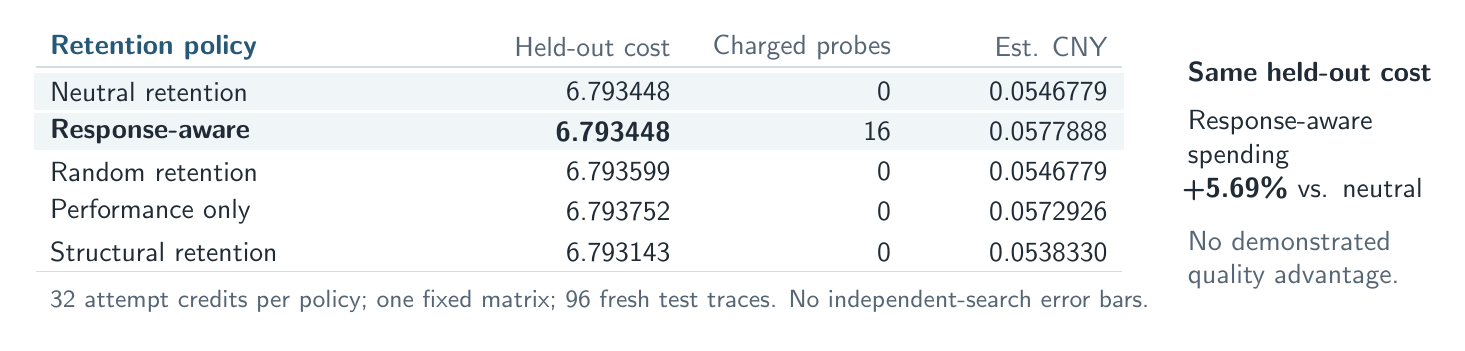
\begin{tikzpicture}[x=1cm,y=1cm,every node/.style={font=\sffamily\fontsize{10}{12}\selectfont,text=ink}]
\path[use as bounding box] (0,0) rectangle (17.9,3.75);
\node[anchor=west,font=\sffamily\bfseries\fontsize{10}{12}\selectfont,text=blue] at (0.15,3.5) {Retention policy};
\node[anchor=east,text=muted] at (8.3,3.5) {Held-out cost};
\node[anchor=east,text=muted] at (11.1,3.5) {Charged probes};
\node[anchor=east,text=muted] at (13.85,3.5) {Est. CNY};
\draw[rulegray] (0.1,3.25)--(13.9,3.25);
\fill[lightblue] (0.08,2.705) rectangle (13.92,3.175);
\node[anchor=west] at (0.15,2.940) {Neutral retention};
\node[anchor=east] at (8.3,2.940) {6.793448};
\node[anchor=east] at (11.1,2.940) {0};
\node[anchor=east] at (13.85,2.940) {0.0546779};
\fill[lightblue] (0.08,2.195) rectangle (13.92,2.665);
\node[font=\sffamily\bfseries\fontsize{10}{12}\selectfont,anchor=west] at (0.15,2.430) {Response-aware};
\node[font=\sffamily\bfseries\fontsize{10}{12}\selectfont,anchor=east] at (8.3,2.430) {6.793448};
\node[anchor=east] at (11.1,2.430) {16};
\node[anchor=east] at (13.85,2.430) {0.0577888};
\node[anchor=west] at (0.15,1.920) {Random retention};
\node[anchor=east] at (8.3,1.920) {6.793599};
\node[anchor=east] at (11.1,1.920) {0};
\node[anchor=east] at (13.85,1.920) {0.0546779};
\node[anchor=west] at (0.15,1.410) {Performance only};
\node[anchor=east] at (8.3,1.410) {6.793752};
\node[anchor=east] at (11.1,1.410) {0};
\node[anchor=east] at (13.85,1.410) {0.0572926};
\node[anchor=west] at (0.15,0.900) {Structural retention};
\node[anchor=east] at (8.3,0.900) {6.793143};
\node[anchor=east] at (11.1,0.900) {0};
\node[anchor=east] at (13.85,0.900) {0.0538330};
\draw[rulegray] (0.1,0.65)--(13.9,0.65);
\node[anchor=north west,text width=3.2cm,align=left,font=\sffamily\fontsize{10}{12.2}\selectfont] at (14.6,3.44) {\textbf{Same held-out cost}\\[5pt]Response-aware spending\\\textbf{+5.69\%} vs. neutral\\[7pt]\color{muted}No demonstrated quality advantage.};
\node[anchor=west,font=\sffamily\fontsize{9.1}{11}\selectfont,text=muted] at (0.15,0.27) {32 attempt credits per policy; one fixed matrix; 96 fresh test traces. No independent-search error bars.};
\end{tikzpicture}

\captionof{figure}{Exact finite-bank expectations at 32 attempt credits; lower cost is better. Values integrate label-balanced descendant subsets and retention randomness on one recorded bank. A numeric display preserves the near-tie without an exaggerated axis. Monetary costs are nominal estimates, not invoices.}
\end{center}

\begin{multicols}{2}
\section{What the comparison establishes}
Response diversity ties neutral retention at 6.793448 with \textbf{5.69\% more} expected generation spending. Structural and shorter-representative controls both score 6.793143. The $+0.000305$ pp response--structural gap does not establish overall structural superiority.

Masked-invalid and complete-valid-pair descriptors, validity flags alone, and the same probes with responses ignored all yield 6.793448. Offspring-quality selection scores 6.793143. The signed descriptor adds no demonstrated predictive value here.

Neither primary budget view has pool censoring. Adding CNY 0.062416 and 30 seconds of measured training evaluation to the 32-attempt ceiling also yields no advantage. Common ceilings permit different realized spending.

\textbf{Statistical unit.} Exact results integrate allocations on \emph{one} parent/offspring matrix. The priced view's 560 allocations are numerical integration, not independent LLM trials. Eight test banks quantify workload variation, not independent searches. Tiny rankings are not significance evidence.

\section{Why the diversity descriptor failed}
An invalid child was encoded as parent cost plus 100 pp. This artificial coordinate contributes \textbf{99.945\%} of the squared distance making \texttt{p06} the first diverse choice: 0.500276 versus 0.005913 for the next parent. Penalties of 0 or 1 pp drop \texttt{p06}; 10, 100 or 1,000 retain it. Masking also drops it. This training-only diagnosis explains that retention decision, not all response differences.

Fresh \texttt{p06} children give no global training improvement. The sole fresh training winner comes from \texttt{p01}, already kept by performance selection. Eight local-edit probes recover the same parent set as sixteen, but their 6.793600 test cost establishes no advantage over free controls.

\section{Interpretation and limits}
The earlier winner's gain did not repeat: 6.800138 versus Best Fit's 6.793143 on fresh traces, with one win, 94 ties and one loss. This limits the original improvement claim without proving universal inferiority. Absolute costs across test sets are not directly comparable.

The contribution is a controlled negative comparison and failure attribution. Semantic neutral drift in genetic programming [2], quality diversity [3] and evolvability [4] already study related distinctions. FunSearch [5] keeps multiple programs per score-signature cluster and favors shorter representatives. Clade-AHD [6] already uses descendant credit. No new algorithm or MetaMuse improvement is established.

Limits include one seed bank, elementary heuristic families, a stateless interface, two reused probe samples per parent and an unpinned provider revision. Neutral retention is one archive-boundary analogue of drift. These are neither multigeneration MetaMuse runs nor reproductions of the cited baselines.

\textbf{Open question.} When can edit-conditioned information repay its acquisition cost beyond neutral, structural and offspring-quality retention? Independent parent banks and frozen, budget-matched tests would be required. Further tuning on these held-out traces is unwarranted.

\section*{References and evidence}
{\fontsize{8.7}{10.5}\selectfont\setlength{\parskip}{2pt}
\refentry{1}{R. Ma, C.-J. M. Liang, Y. Gao and F. Y. Yan. \href{https://proceedings.iclr.cc/paper_files/paper/2026/hash/85632be2cd69e9a0ef4ba054c096fac9-Abstract-Conference.html}{MetaMuse: Algorithm Generation via Creative Ideation}. ICLR, 2026.}
\refentry{2}{T. Atkinson, D. Plump and S. Stepney. \href{https://doi.org/10.1007/s11047-019-09772-4}{Evolving graphs with semantic neutral drift}. \emph{Natural Computing} 20:127--143, 2021.}
\refentry{3}{J.-B. Mouret and J. Clune. \href{https://arxiv.org/abs/1504.04909}{Illuminating search spaces by mapping elites}. arXiv:1504.04909, 2015.}
\refentry{4}{A. Katona, D. W. Franks and J. A. Walker. \href{https://arxiv.org/abs/2103.10790v1}{Quality Evolvability ES: Evolving Individuals With a Distribution of Well Performing and Diverse Offspring}. arXiv:2103.10790v1, 2021.}
\refentry{5}{B. Romera-Paredes et al. \href{https://doi.org/10.1038/s41586-023-06924-6}{Mathematical discoveries from program search with large language models}. \emph{Nature} 625:468--475, 2024.}
\refentry{6}{K. Lai, Y. Lai and H.-L. Liu. \href{https://arxiv.org/abs/2602.00549v1}{Beyond the Node: Clade-level Selection for Efficient MCTS in Automatic Heuristic Design}. arXiv:2602.00549v1, 2026.}
\par\vspace{3pt}{\raggedright\textbf{Code and reproducibility.}\\
\href{https://github.com/ZhijingWu/metamuse-edit-response-study}{\nolinkurl{github.com/ZhijingWu/metamuse-edit-response-study}}\\
Frozen protocols, executable evaluation code and shareable experimental artifacts are available in the repository.\par}}
\end{multicols}
\end{document}
